% % \begin{figure}
% % 	\centering
% 	\begin{minipage}{.5\textwidth}
% 		\centering
% 		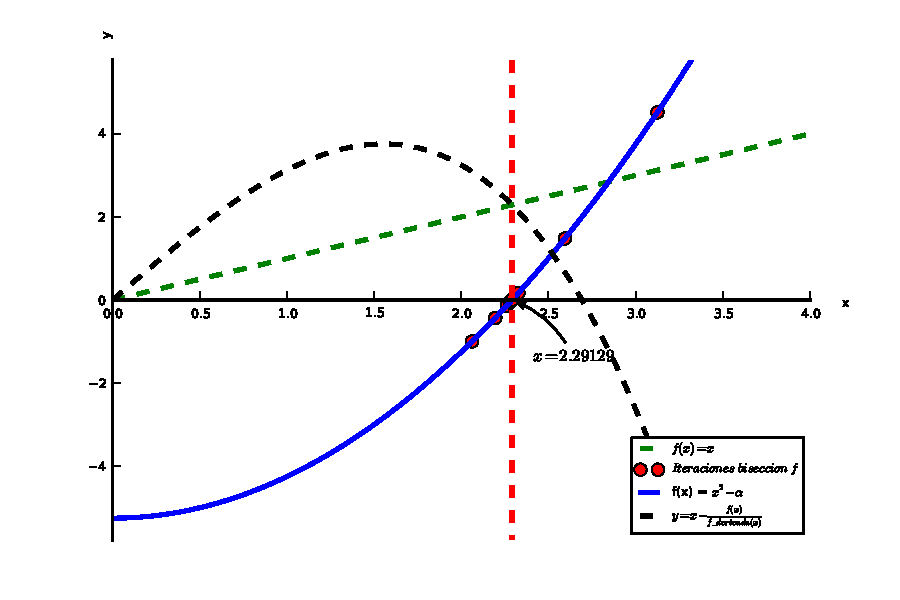
\includegraphics[keepaspectratio]{Imagenes/exp1/biseccion_f.pdf}
% 		\captionof{figure}{A figure}
% 		\label{fig:test1}
% 	\end{minipage}%
% 	\begin{minipage}{.5\textwidth}
% 		\centering
% 		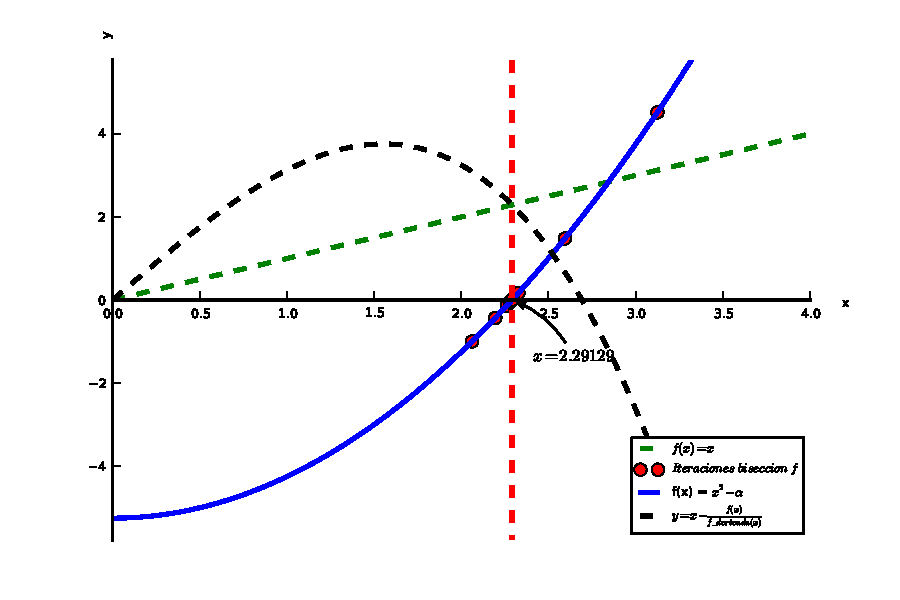
\includegraphics[keepaspectratio]{Imagenes/exp1/biseccion_f.pdf}
% 		\captionof{figure}{Another figure}
% 		\label{fig:test2}
% 	\end{minipage}
% \end{figure}

\begin{figure}[!h]
	\begin{center}
		  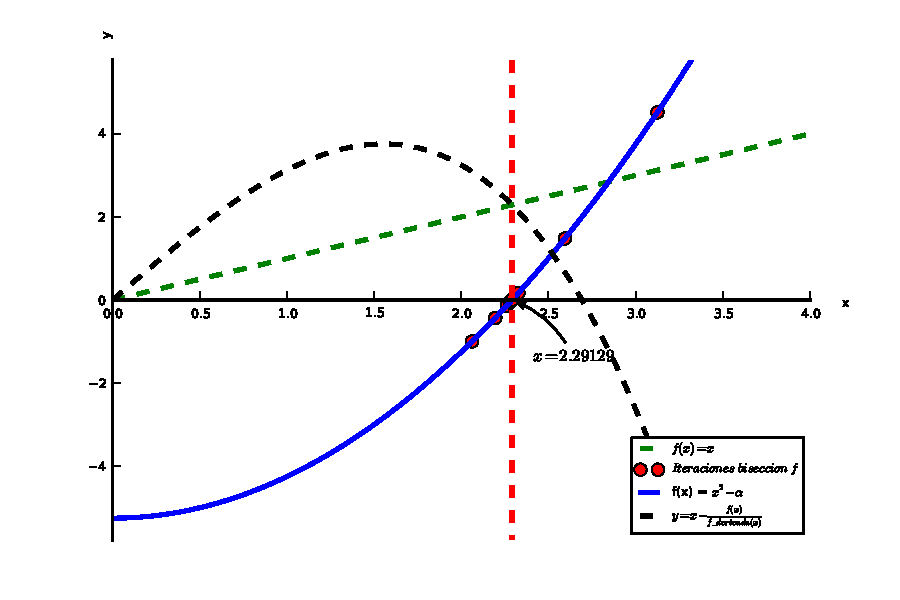
\includegraphics[keepaspectratio]{Imagenes/exp1/biseccion_f.pdf}
		  \caption{Bisección\_f para $\alpha=5.25, \epsilon = 1*10^{-5}, criterio = 3$}
		  \label{fig:contra1}
	\end{center}
\end{figure}

~

\begin{figure}[!h]
	\begin{center}
		  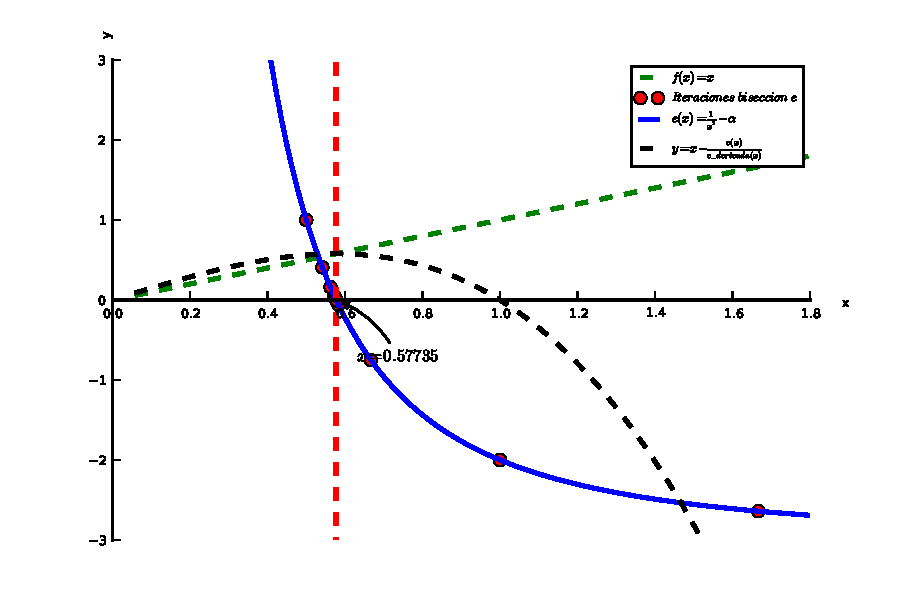
\includegraphics[keepaspectratio]{Imagenes/exp1/biseccion_e.pdf}
		  \caption{Bisección\_e para $\alpha=3.0, \epsilon = 1*10^{-5}, criterio = 1$}
		  \label{fig:contra1}
	\end{center}
\end{figure}

